\documentclass[conference]{IEEEtran}
\IEEEoverridecommandlockouts
\usepackage{cite}
\usepackage{amsmath,amssymb}
\usepackage{graphicx}
\usepackage{booktabs}
\usepackage{multirow}
\usepackage{array}
\usepackage{url}
\usepackage[hidelinks]{hyperref}
\usepackage{tikz}
\usepackage{pgfplots}
\usepackage{xcolor}
\usepackage{listings}
\usetikzlibrary{positioning,arrows.meta,shapes.geometric,fit,calc}
\pgfplotsset{compat=1.18}
\hypersetup{hidelinks}
\definecolor{codegray}{gray}{0.95}
\lstset{basicstyle=\ttfamily\scriptsize,breaklines=true,backgroundcolor=\color{codegray},frame=single}
\sloppy
\setlength{\tabcolsep}{0.5pt}

\title{An Evidence-Centric Pipeline for Real-Time AI Governance Monitoring}

\author{\IEEEauthorblockN{Aditya Ranjan, Arindam Gupta, Gnanendra Naidu N, Dr. S. Anupama Kumar, and Dr. Vijayalakshmi M.N.}
\IEEEauthorblockA{Department of Artificial Intelligence and Machine Learning\\
RV College of Engineering, Bengaluru, India\\
\texttt{adityaranjan.ai23@rvce.edu.in}, \texttt{arindamgupta.ai23@rvce.edu.in},\\
\texttt{gnanendran.ai23@rvce.edu.in}, \texttt{anupamakumar@rvce.edu.in},\\
\texttt{vijayalakshmi@rvce.edu.in}}}

\begin{document}
\maketitle

\begin{abstract}
AI governance evidence is distributed across identity systems, infrastructure logs, data pipelines, model registries, and large-language-model gateways. This paper presents a runnable reference pipeline that converts those heterogeneous events into durable, inspectable governance findings. Five HTTP producer adapters normalize source events into a versioned contract and publish to dedicated Kafka topics. A Kafka Streams topology applies sixteen deterministic controls, event-time windows, state stores, and model-evidence joins. A risk service combines a severity-frequency baseline with an online Isolation Forest comparison, while PostgreSQL preserves events, findings, evidence, scores, agent jobs, and reviews. Two bounded Amazon Bedrock agents investigate and review evidence without performing remediation. The implementation is evaluated using repository-provided functional and recovery demonstrations: 72 labelled events produced 48 expected findings across sixteen rules, with all expected findings recovered in baseline, processor-replacement, and broker-restart scenarios. The paper contributes an end-to-end systems design, explicit recovery boundaries, and an evidence model that connects detection, scoring, review, and reporting while distinguishing engineering evidence from legal conformity.
\end{abstract}

\begin{IEEEkeywords}
AI governance, Kafka Streams, event-time processing, audit evidence, risk scoring, Isolation Forest, agentic AI, PostgreSQL
\end{IEEEkeywords}

\section{Introduction}
AI systems are now operated as socio-technical services rather than isolated models. Governance evidence is consequently generated by many components: identity providers emit access events, Kubernetes emits audit records, orchestration systems emit lineage events, model registries expose lifecycle transitions, and LLM gateways expose prompt and tool activity. A governance team that receives these records without a common contract must manually reconstruct which control was triggered, what evidence supports it, how severe the result is, and whether an investigator has reviewed it. The result is a gap between governance principles and operationally verifiable evidence.

Recent guidance describes AI risk management as a lifecycle activity involving accountability, measurement, monitoring, documentation, and human oversight [1]--[6]. Security taxonomies add prompt injection, data leakage, excessive agency, and supply-chain risks for AI-enabled applications [7], [8]. These sources establish what should be governed, but they do not provide a complete streaming implementation for correlating heterogeneous producer activity with durable findings, comparative risk signals, and bounded agent review.

This paper presents the AI-Governance-Audit-Pipeline, a repository-backed reference implementation. Its design goals are: (i) normalize heterogeneous events without losing provenance; (ii) evaluate executable controls with event-time and stateful processing; (iii) preserve a reconstructable audit trail; (iv) add risk scoring without hiding the deterministic policy result; and (v) use agents as advisory, evidence-grounded workers with bounded revision and human escalation. The implementation is deliberately described as a reference architecture, not as proof of regulatory conformity or general model accuracy.

The main contributions are an integrated event-to-evidence architecture, a Kafka topology that combines windows and joins for governance controls, a dual baseline/ML risk model, and a bounded two-agent review protocol. The remainder of the paper describes the related literature, system requirements, architecture, implementation, evaluation, limitations, and future work.

\section{Related Work and Research Gap}
\subsection{Governance and operational evidence}
NIST AI RMF 1.0 organizes risk work around govern, map, measure, and manage functions [1]. Its GenAI Profile adds risks and actions specific to generative systems [2]. ISO/IEC 42001 frames AI governance as a management system with ownership and continual improvement [3]. The OECD principles and UNESCO recommendation emphasize accountability, transparency, human oversight, and human-centred values [4], [5]. The EU AI Act introduces a risk-tiered regulatory setting [6]. Collectively, these works motivate explicit ownership, traceability, and review states.

The operational gap is that principles and obligations do not identify the telemetry path needed to produce an auditable case. A practical system must correlate source activity, control logic, evidence, score, reviewer outcome, and revision history. This paper treats that correlation path as a systems problem.

\subsection{Security, streaming, and agents}
OWASP's LLM application risks and MITRE ATLAS techniques provide security-oriented taxonomies [7], [8]. Google SAIF and OpenSSF Scorecard address secure development and software supply-chain practices [9], [10]. Kafka Streams provides event-time state, windows, joins, and recovery semantics [11], while Kubernetes supplies operational patterns for probes, scaling, and disruptions [12]. Retrieval-augmented generation surveys emphasize grounding and evaluation [13], and agent surveys identify planning, tools, memory, and control as central design concerns [14].

The gap is not the absence of individual techniques. It is the lack of an end-to-end evidence path that combines the techniques under a single identity and persistence model. The proposed pipeline addresses this gap by storing source, finding, score, evidence, agent report, review, and audit-history identifiers in one operational system.

\begin{table}[t]
\caption{Positioning against recent work}
\label{tab:related}
\centering\scriptsize
\begin{tabular}{p{1.35cm}p{1.55cm}p{2.05cm}p{1.85cm}}
\toprule
\textbf{Source} & \textbf{Method/data} & \textbf{Key contribution} & \textbf{Gap addressed here}\\
\midrule
NIST [1], [2] & Risk frameworks and lifecycle guidance & Govern, map, measure, manage & Executable event-to-control path\\
ISO/OECD [3], [4] & Management-system and policy principles & Ownership, transparency, improvement & Durable implementation evidence\\
OWASP / MITRE [7], [8] & AI security taxonomies & Threat and abuse coverage & Correlated findings and review\\
Kafka / Kubernetes [11], [12] & Streaming and operations mechanisms & State, joins, recovery, scaling & Governance-specific topology\\
RAG/agent surveys [13], [14] & Retrieval and autonomous-agent synthesis & Grounding and bounded action concerns & Evidence-cited agent workflow\\
\bottomrule
\end{tabular}
\end{table}

\section{System Requirements and Design}
The repository defines five producer domains: Keycloak identity, Kubernetes audit, Airflow/OpenLineage pipeline activity, model registry activity, and an LLM gateway. Each adapter exposes health, readiness, metrics, and ingestion endpoints, validates source-specific payloads, maps them into the canonical governance-event schema, and publishes to a dedicated raw topic. This isolation permits source-specific evolution without weakening the downstream contract.

The stream processor must support stateless controls and stateful controls. Stateless controls evaluate an event independently. Stateful controls require event-time accumulation or relationships among records: a failed-login burst needs a window, while an unsafe model promotion needs approval and evaluation evidence joined before a promotion event is assessed. Findings require stable keys so downstream services can correlate scores and stored evidence.

The persistence boundary must be idempotent. A replayed event should not create an unbounded set of duplicate events or findings. The database therefore stores event identifiers, finding identifiers, evidence records, score fields, agent jobs, reports, reviews, and audit history. Consumers are separated so scoring or reporting lag does not block detection.

\subsection{Canonical event contract}
The canonical event is the principal abstraction that allows five source domains to share one downstream topology. It carries a schema version, event identifier, producer, event timestamp, ingestion timestamp, actor, object, action, attributes, and evidence metadata. Source adapters retain source-specific identifiers inside the attributes and evidence fields rather than discarding them during normalization. This lets a reviewer inspect the normalized event used by a rule while still returning to the source identifier during investigation.

The contract separates event time from processing time. The event timestamp is used by Kafka Streams for windows and joins; the ingestion timestamp describes when the platform received the record. A delayed record can therefore be evaluated according to the business timestamp rather than silently becoming a new event. Adapter validation rejects malformed records before they enter the primary stream.

\begin{table}[t]\caption{Canonical governance-event fields}\label{tab:contract}\centering\scriptsize\begin{tabular}{p{1.55cm}p{2.6cm}p{2.3cm}}\toprule\textbf{Field group} & \textbf{Representative fields} & \textbf{Audit purpose}\\\midrule Identity & schema version, event ID, producer & Compatibility and deduplication\\ Time & event time, ingestion time & Event-time processing and latency\\ Actor/object & actor ID, object type, object ID & Subject and resource correlation\\ Action & action, outcome, severity & Rule predicates and risk baseline\\ Attributes & source-specific key/value data & Preserve producer context\\ Evidence & source reference, raw metadata & Reproducible review and provenance\\\bottomrule\end{tabular}\end{table}

\begin{figure}[t]
\centering
\resizebox{\columnwidth}{!}{%
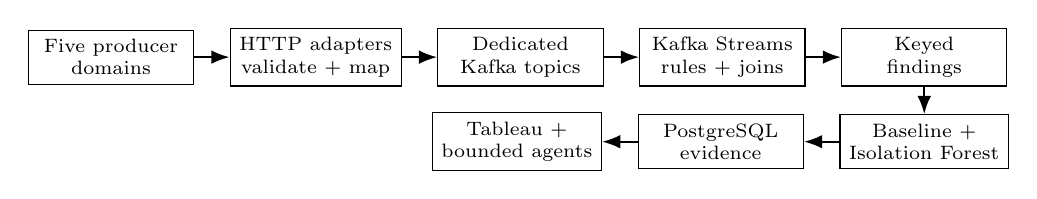
\begin{tikzpicture}[box/.style={draw,align=center,minimum height=0.65cm,minimum width=2.1cm,font=\scriptsize},arr/.style={-Latex,thick},node distance=0.35cm and 0.45cm]
\node[box] (src) {Five producer\\domains};
\node[box,right=of src] (adp) {HTTP adapters\\validate + map};
\node[box,right=of adp] (raw) {Dedicated\\Kafka topics};
\node[box,right=of raw] (top) {Kafka Streams\\rules + joins};
\node[box,right=of top] (find) {Keyed\\findings};
\node[box,below=of find] (score) {Baseline +\\Isolation Forest};
\node[box,left=of score] (db) {PostgreSQL\\evidence};
\node[box,left=of db] (out) {Tableau +\\bounded agents};
\draw[arr] (src)--(adp); \draw[arr] (adp)--(raw); \draw[arr] (raw)--(top); \draw[arr] (top)--(find); \draw[arr] (find)--(score); \draw[arr] (score)--(db); \draw[arr] (db)--(out);
\end{tikzpicture}}
\caption{End-to-end architecture and evidence boundary.}
\label{fig:architecture}
\end{figure}

\section{Kafka Streams Processing Design}
\subsection{Topics, keys, and event time}
The local configuration creates six partitions per topic and runs two Kafka Streams threads; the AWS configuration uses a three-broker MSK cluster, replication factor three, and a minimum in-sync replica policy. Producer topics separate contracts, while keys are selected for the state operation: actor identifiers support failed-login windows, model identifiers support approval/evaluation joins, and finding identifiers support downstream correlation.

An event timestamp extractor makes the event time explicit. The failed-login rule uses a five-minute window with a one-minute grace period. A record arriving after the event-time boundary can therefore be classified according to the business timestamp rather than arrival order, while the grace period limits how long state remains open.

\subsection{State stores and joins}
The topology materializes approval state, evaluation state, combined model-governance evidence, and failed-login state. A table-table outer join combines approval and evaluation records even when one side arrives first. A stream-table left join checks a production promotion against the combined model evidence. Stateless findings and stateful findings are merged into a raw-finding topic, where the finding ID becomes the output key. JSON serializers preserve a typed but human-readable contract.

\begin{table}[t]
\caption{Kafka features incorporated in the implementation}
\label{tab:kafka}
\centering\tiny
\begin{tabular}{p{1.7cm}p{2.5cm}p{2.2cm}}
\toprule
\textbf{Feature} & \textbf{Implementation} & \textbf{Benefit}\\
\midrule
Topics & One raw topic per producer & Contract isolation\\
Partitions/keys & Six partitions; actor, model, finding keys & Parallelism and correlation\\
Event time & Timestamp extractor, 5-min window, 1-min grace & Late-event correctness\\
State/joins & Materialized tables and stream-table join & Evidence composition\\
Groups & Rules, scoring, persistence, evaluation groups & Independent replay\\
Durability & MSK RF 3, minimum ISR 2 & Restart recovery\\
Serialization & JSON serdes & Versioned readable records\\
\bottomrule
\end{tabular}
\end{table}

\subsection{Rule catalogue and framework mapping}
The repository configures sixteen executable rules and maps each rule to governance frameworks including NIST AI RMF, ISO/IEC 42001, the EU AI Act, NIST SP 800-53, and GDPR. The mapping is stored with the finding as descriptive metadata. It helps a reviewer route a finding to an accountable control owner, but it is not treated as an automated legal conclusion.

The rules cover both security-oriented and lifecycle-oriented conditions. Examples include failed-login bursts, model approval and evaluation relationships, promotion without required evidence, pipeline or registry conditions, and LLM gateway observations. A rule result includes rule identity, severity, triggering event identity, timestamps, framework labels, and evidence references. Keeping the rule identifier in the finding makes the result explainable: a reviewer can locate the configured condition and compare it with the triggering event.

The stateful rules are especially important because governance evidence is often distributed across time. A model approval and its evaluation may arrive as separate records; a promotion may arrive after both. A five-minute failed-login rule similarly depends on a sequence rather than one record. Windows, state stores, joins, and grace periods make these conditions explicit instead of forcing downstream operators to infer them from raw logs.

\begin{figure}[t]
\centering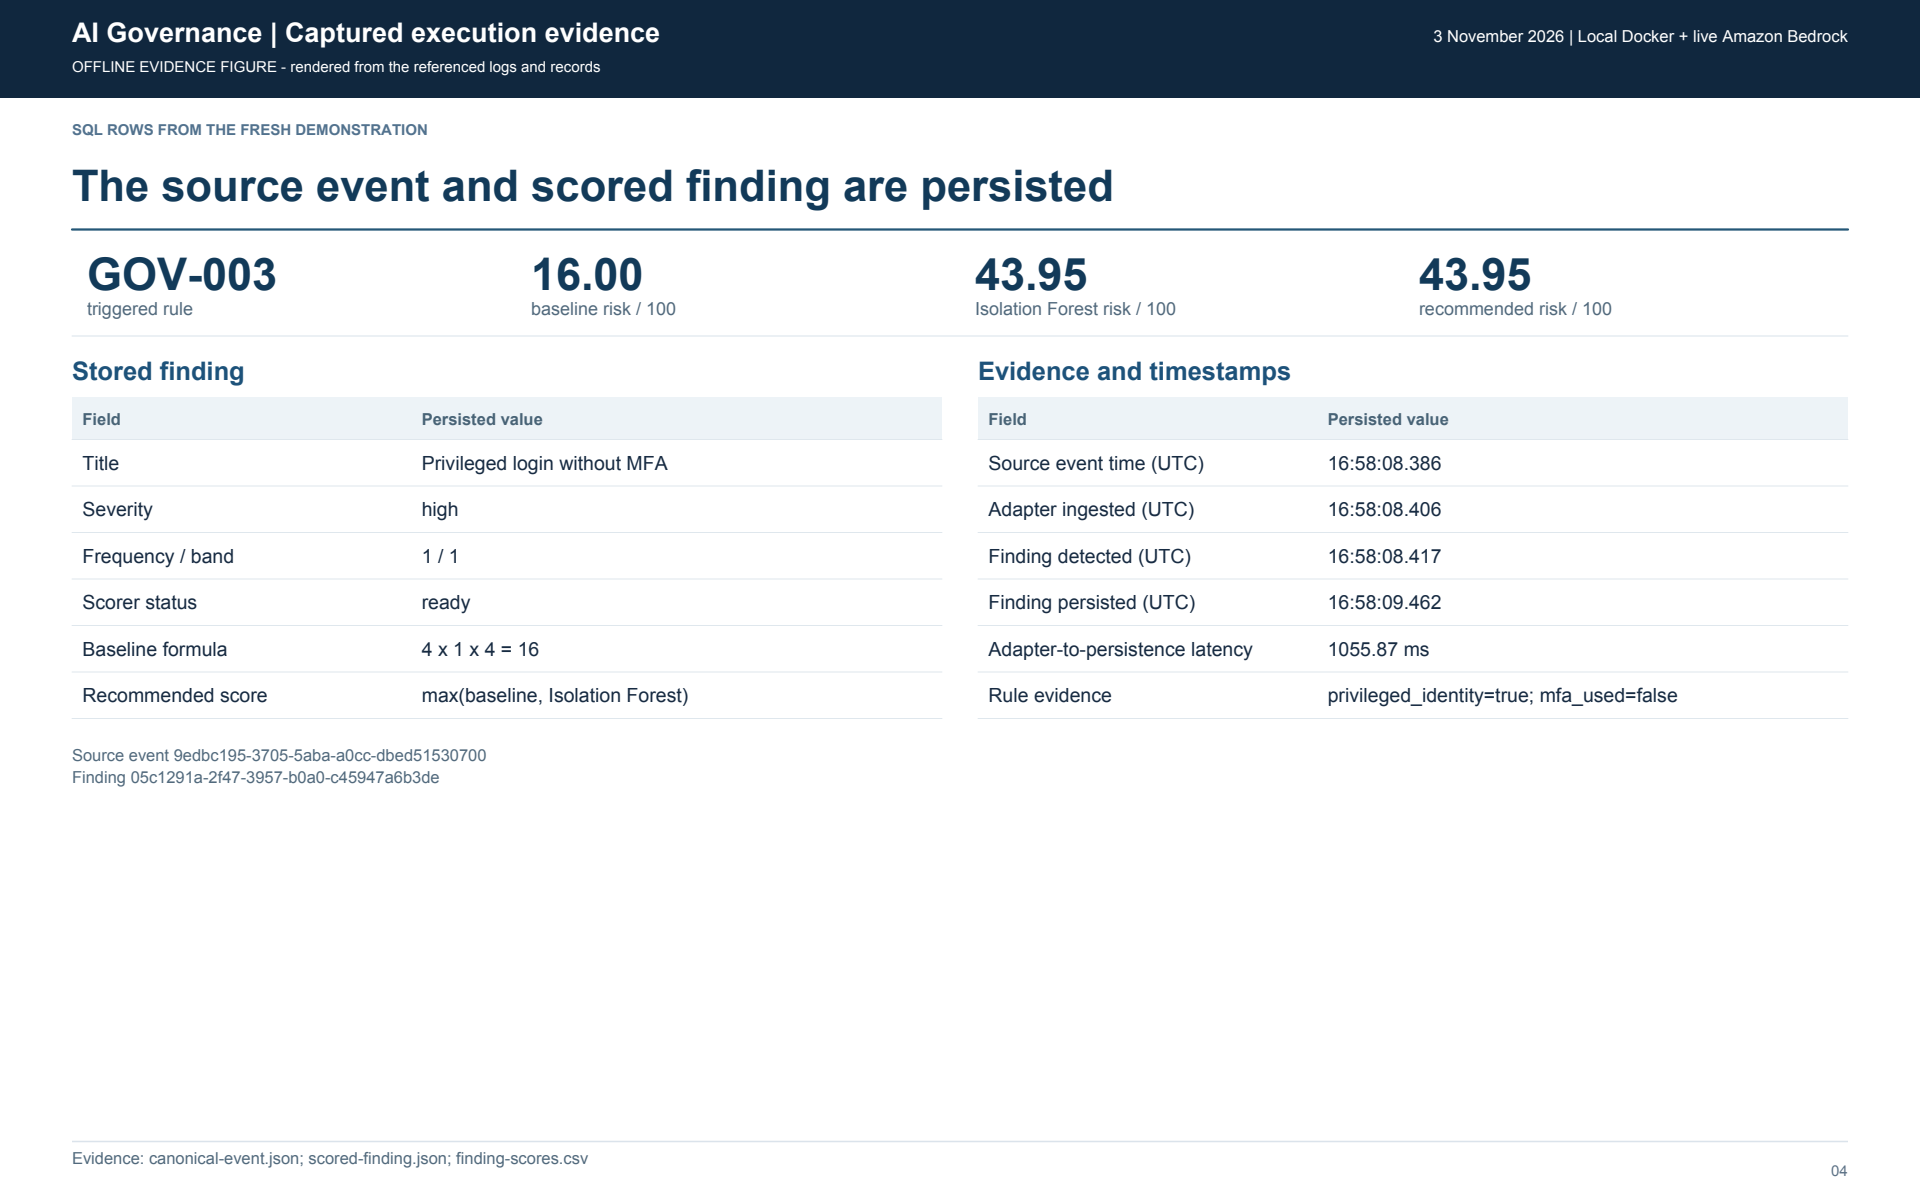
\includegraphics[width=\columnwidth]{figures/04-persisted-finding.png}
\caption{Persisted finding with rule, triggering event, score, and timestamps.}
\label{fig:finding}
\end{figure}

\section{Risk Scoring and Agent Workflow}
The deterministic baseline combines severity and frequency. If $s\in[1,5]$ is severity and $f\in[1,5]$ is the frequency bucket, the baseline is computed as
\begin{equation}
 B = 20(0.6s+0.4f).
\end{equation}
The service additionally maintains an online Isolation Forest over recent finding features including severity, frequency, baseline risk, time-of-day, rule identity, and producer type. The model begins training after 32 findings, retrains after each 25 additional findings, and retains at most 1,000 recent findings. When ready, the recommended score is the higher of the baseline and ML scores, preserving a conservative deterministic floor.

The Investigator retrieves eligible evidence and writes a structured report. The Evidence Reviewer checks evidence citations and completeness, requests at most one correction, and may terminate with a human-review status. Neither agent remediates infrastructure. Reports and evidence snapshots are retained as durable records, so the agent output is inspectable rather than an ephemeral chat response.

\subsection{Risk interpretation and control boundary}
The score is not a replacement for the governance rule. The rule explains why an event was selected; the score prioritizes the finding for operational attention. The baseline remains available when the Isolation Forest is not ready, including cold start and post-deployment periods. The scorer records readiness, baseline score, ML score, score delta, and recommended score, allowing a reviewer to distinguish policy severity from statistical unusualness.

The feature set includes severity, frequency, baseline risk, time of day, rule identity, and producer type. The unsupervised signal is comparative rather than a claim that the model understands legal or organizational risk. This separation limits the risk that a statistical signal is mistaken for a policy decision. The agents operate only after evidence exists: the Investigator retrieves records, the Reviewer checks citations and completeness, and a bounded correction can terminate in human review.

\begin{figure}[t]
\centering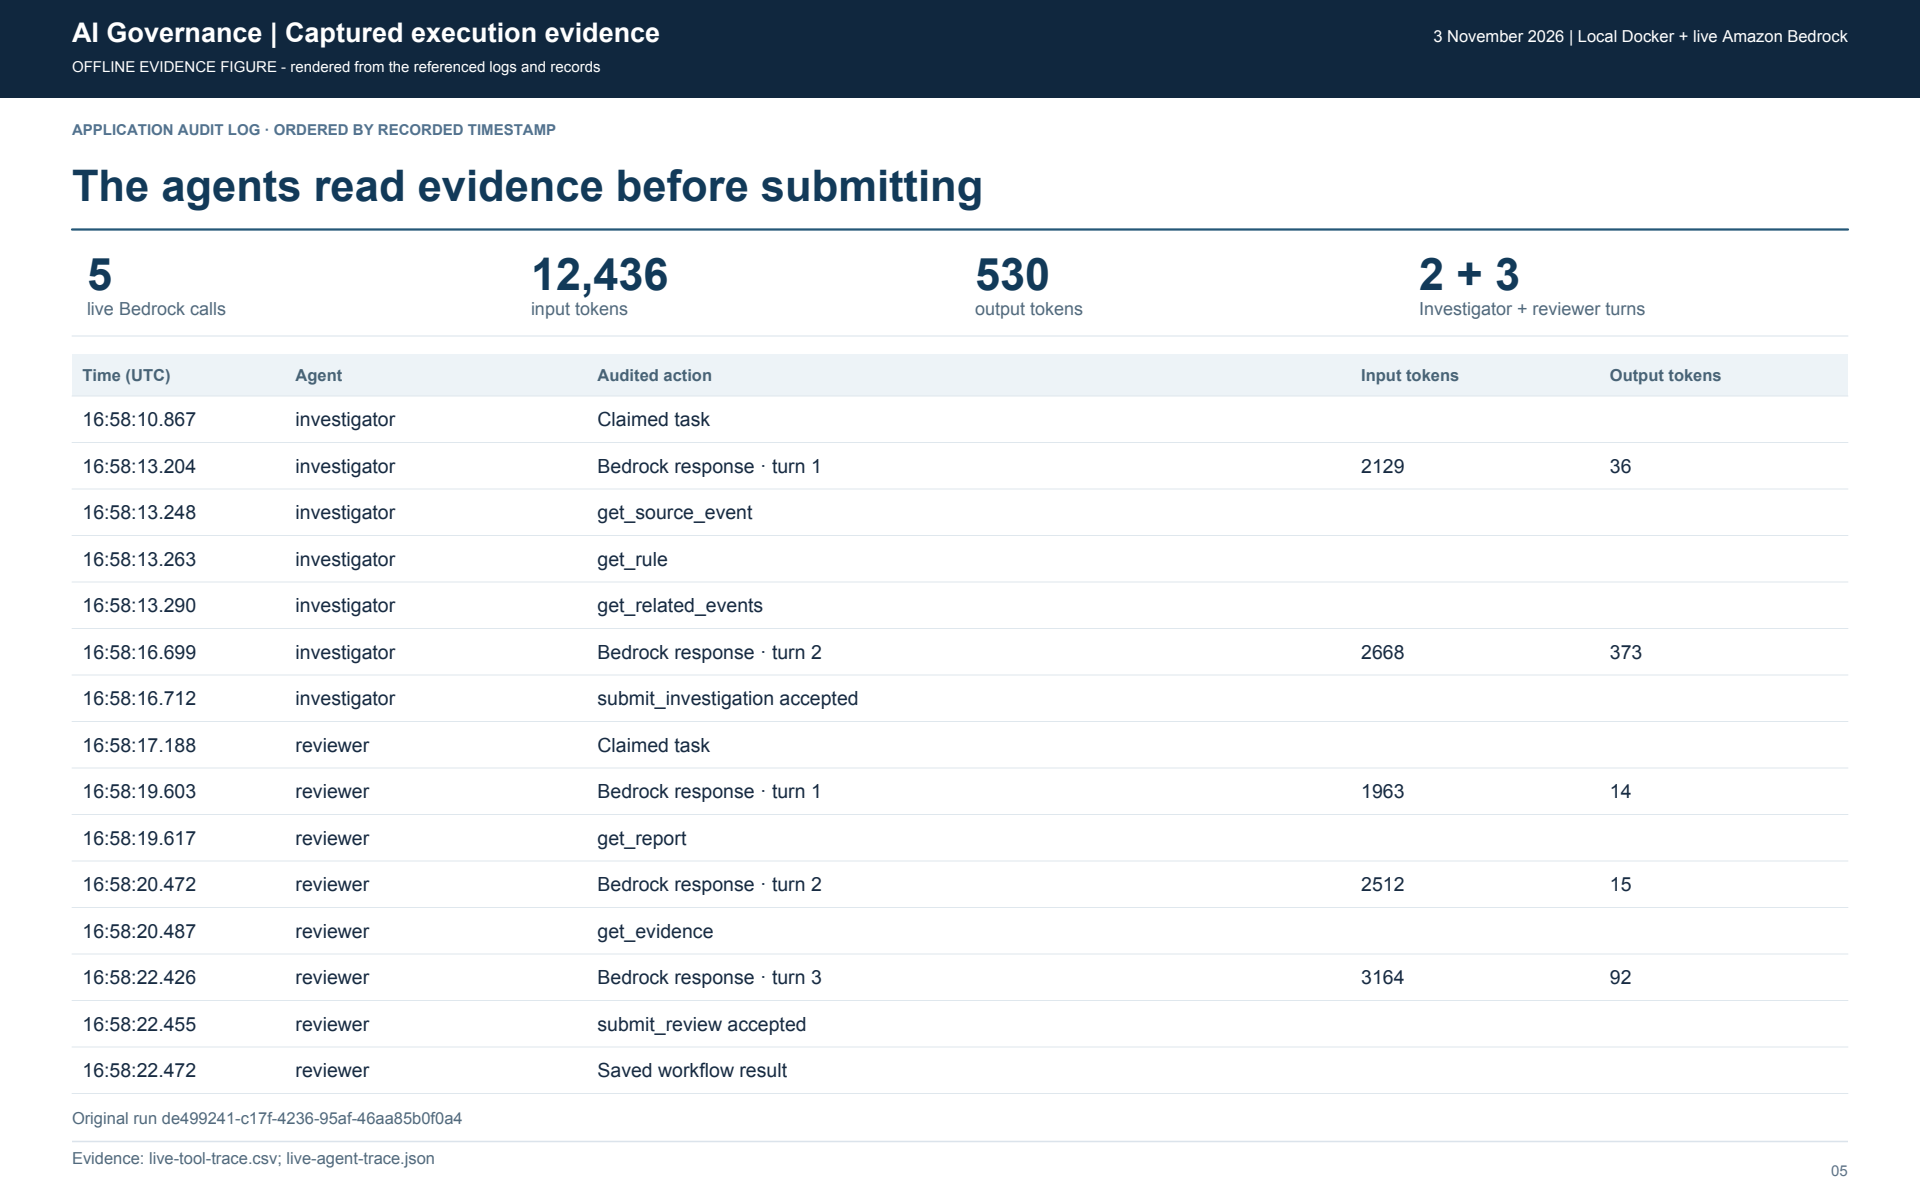
\includegraphics[width=\columnwidth]{figures/05-agent-tool-trace.png}
\caption{Repository evidence of the Investigator and Evidence Reviewer tool trace.}
\label{fig:agents}
\end{figure}

\section{Implementation and Deployment}
The repository contains Java source for the Kafka Streams topology and rule engine, Python services for adapters, scoring, persistence, investigation, review, and evaluation, SQL migrations for the evidence model, Docker Compose for local execution, Kubernetes manifests for service deployment, and Terraform for AWS infrastructure. The local profile uses Redpanda as a Kafka-compatible broker and PostgreSQL as the durable store. The cloud profile provisions MSK, EKS, RDS, ECR, IAM, VPC, and security-group resources.

The implementation separates detection, scoring, persistence, and evaluation consumer groups. This design permits replay from independent committed offsets and prevents a reporting slowdown from blocking rule detection. Idempotent database writes provide a second protection against replay duplication. Health, readiness, metrics, and operational pause/resume scripts make failure handling explicit.

\subsection{Service boundaries and recovery}
The five adapters are independently deployable services with their own images, health endpoints, readiness endpoints, metrics, and producer settings. The Java stream processor contains the event, finding, evidence, promotion, login-burst, and rule models. Python services provide scoring, persistence, investigation, review, and evaluation. A producer can restart without stopping stream processing; the processor can be replaced while records remain in Kafka; the scorer and sink can replay from independent consumer groups.

The local profile uses Docker Compose, Redpanda, and PostgreSQL. The AWS profile uses Terraform for VPC, MSK, EKS, RDS, ECR, IAM, and security groups, with Kubernetes manifests for deployments, services, probes, scaling, and disruption budgets. The two profiles are intentionally distinguished: local measurements demonstrate functional behaviour, while cloud resources provide a deployment path and observability rather than a production capacity claim.

Recovery is tested at three layers. Kafka retains records and offsets, Kafka Streams rebuilds state from its input history, and PostgreSQL idempotency prevents replayed records from multiplying durable rows. At the workflow layer, corrected reports do not erase original evidence. A recovery pass is therefore defined as restoration of the expected finding set, not merely process liveness.

\begin{figure}[t]
\centering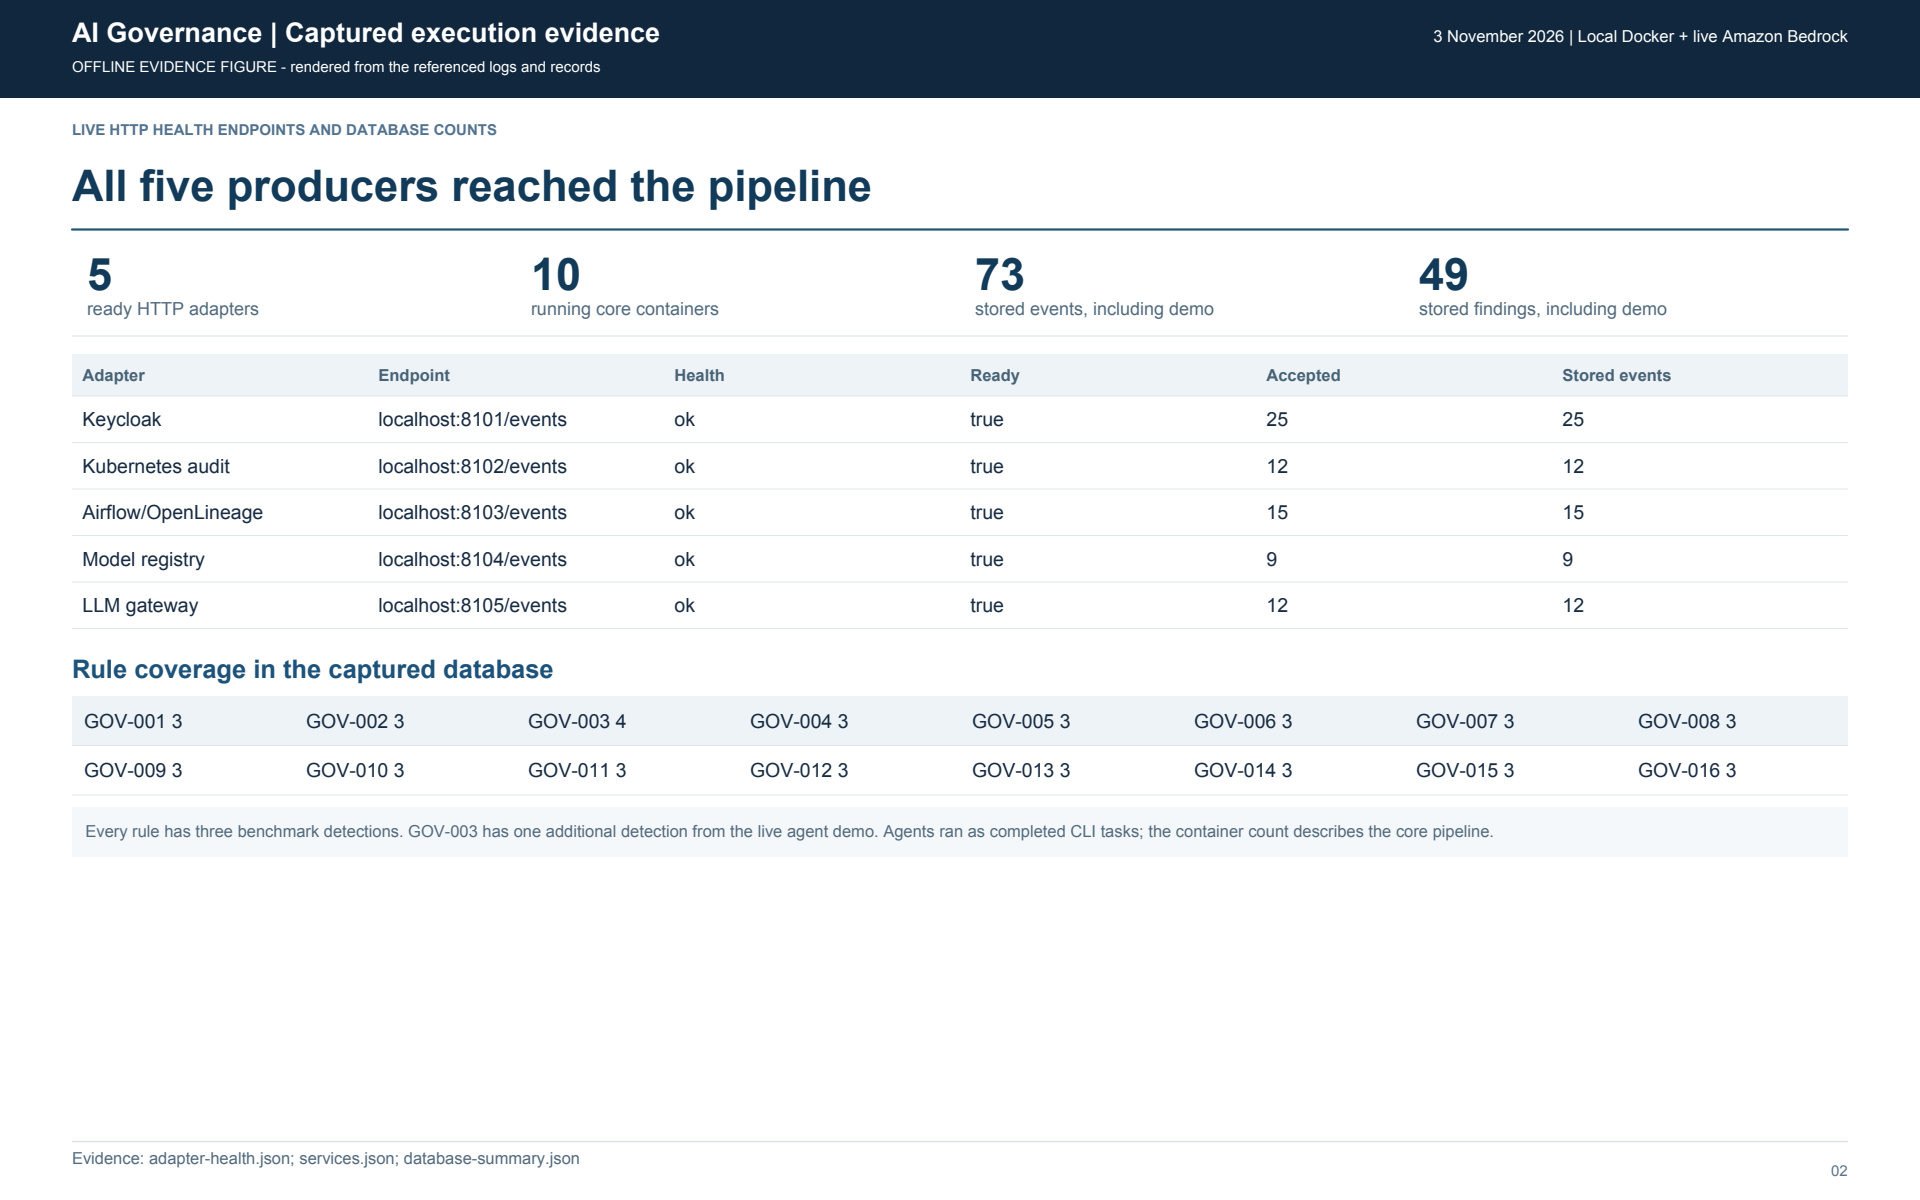
\includegraphics[width=\columnwidth]{figures/02-producer-health.png}
\caption{Producer adapter health and accepted-event evidence.}
\label{fig:producers}
\end{figure}

\section{Evaluation}
The repository evaluation uses source-shaped synthetic events and a labelled expected-finding set. The main demonstration contains 72 events and 48 expected findings across all 16 rules. Four scenarios are reported: baseline execution, processor replacement, broker restart, and independent adapters. The evaluation checks expected finding recovery, precision and recall against the labelled expectation, throughput, and persistence behaviour.

\subsection{Evaluation protocol}
For each scenario, the evaluator injects source-shaped events, waits for the pipeline to settle, consumes the finding output, and compares observed finding identities against the expected set. Precision and recall are computed over the labelled workload. Throughput and latency are reported for the observed injection or persistence interval. Additional checks inspect consumer tails, PostgreSQL records, recovery behaviour, and agent terminal states, making the evaluation broader than a single end-to-end count.

\begin{table}[t]
\caption{Repository-reported functional and recovery results}
\label{tab:results}
\centering\scriptsize
\begin{tabular}{lrrrrr}
\toprule
\textbf{Scenario} & \textbf{Events} & \textbf{Exp./Obs.} & \textbf{Prec.} & \textbf{Recall} & \textbf{Rate}\\
\midrule
Baseline & 72 & 48/48 & 1.000 & 1.000 & 130.90/s\\
Processor replacement & 72 & 48/48 & 1.000 & 1.000 & 11.50/s\\
Broker restart & 72 & 48/48 & 1.000 & 1.000 & 11.48/s\\
Independent adapters & 72 & 48/48 & 1.000 & 1.000 & 667.12/s\\
\bottomrule
\end{tabular}
\end{table}

The fresh evidence package reports p50 latency of 353.84 ms, p95 of 1,878.88 ms, p99 of 2,181.69 ms, and 39.04 events/s over the observed persistence interval. These values describe the labelled local workload and should not be interpreted as production capacity or general model accuracy. The evidence also records recovery checks, consumer-tail checks, database persistence, and agent review outcomes.

\begin{table}[t]\caption{Evaluation dimensions and evidence}\label{tab:eval}\centering\scriptsize\begin{tabular}{p{1.7cm}p{2.5cm}p{2.15cm}}\toprule\textbf{Dimension} & \textbf{Measurement} & \textbf{Evidence source}\\\midrule Detection & Expected versus observed findings & Labelled evaluator output\\ Recovery & Finding-set preservation after restart & Resilience scenarios\\ Persistence & Event, finding, and evidence rows & PostgreSQL checks\\ Streaming & Consumer delivery and latency & Kafka output and metrics\\ Agents & Citation, revision, terminal state & Reviewer records\\ Reporting & Risk and framework views & Tableau evidence\\\bottomrule\end{tabular}\end{table}

\begin{figure}[t]
\centering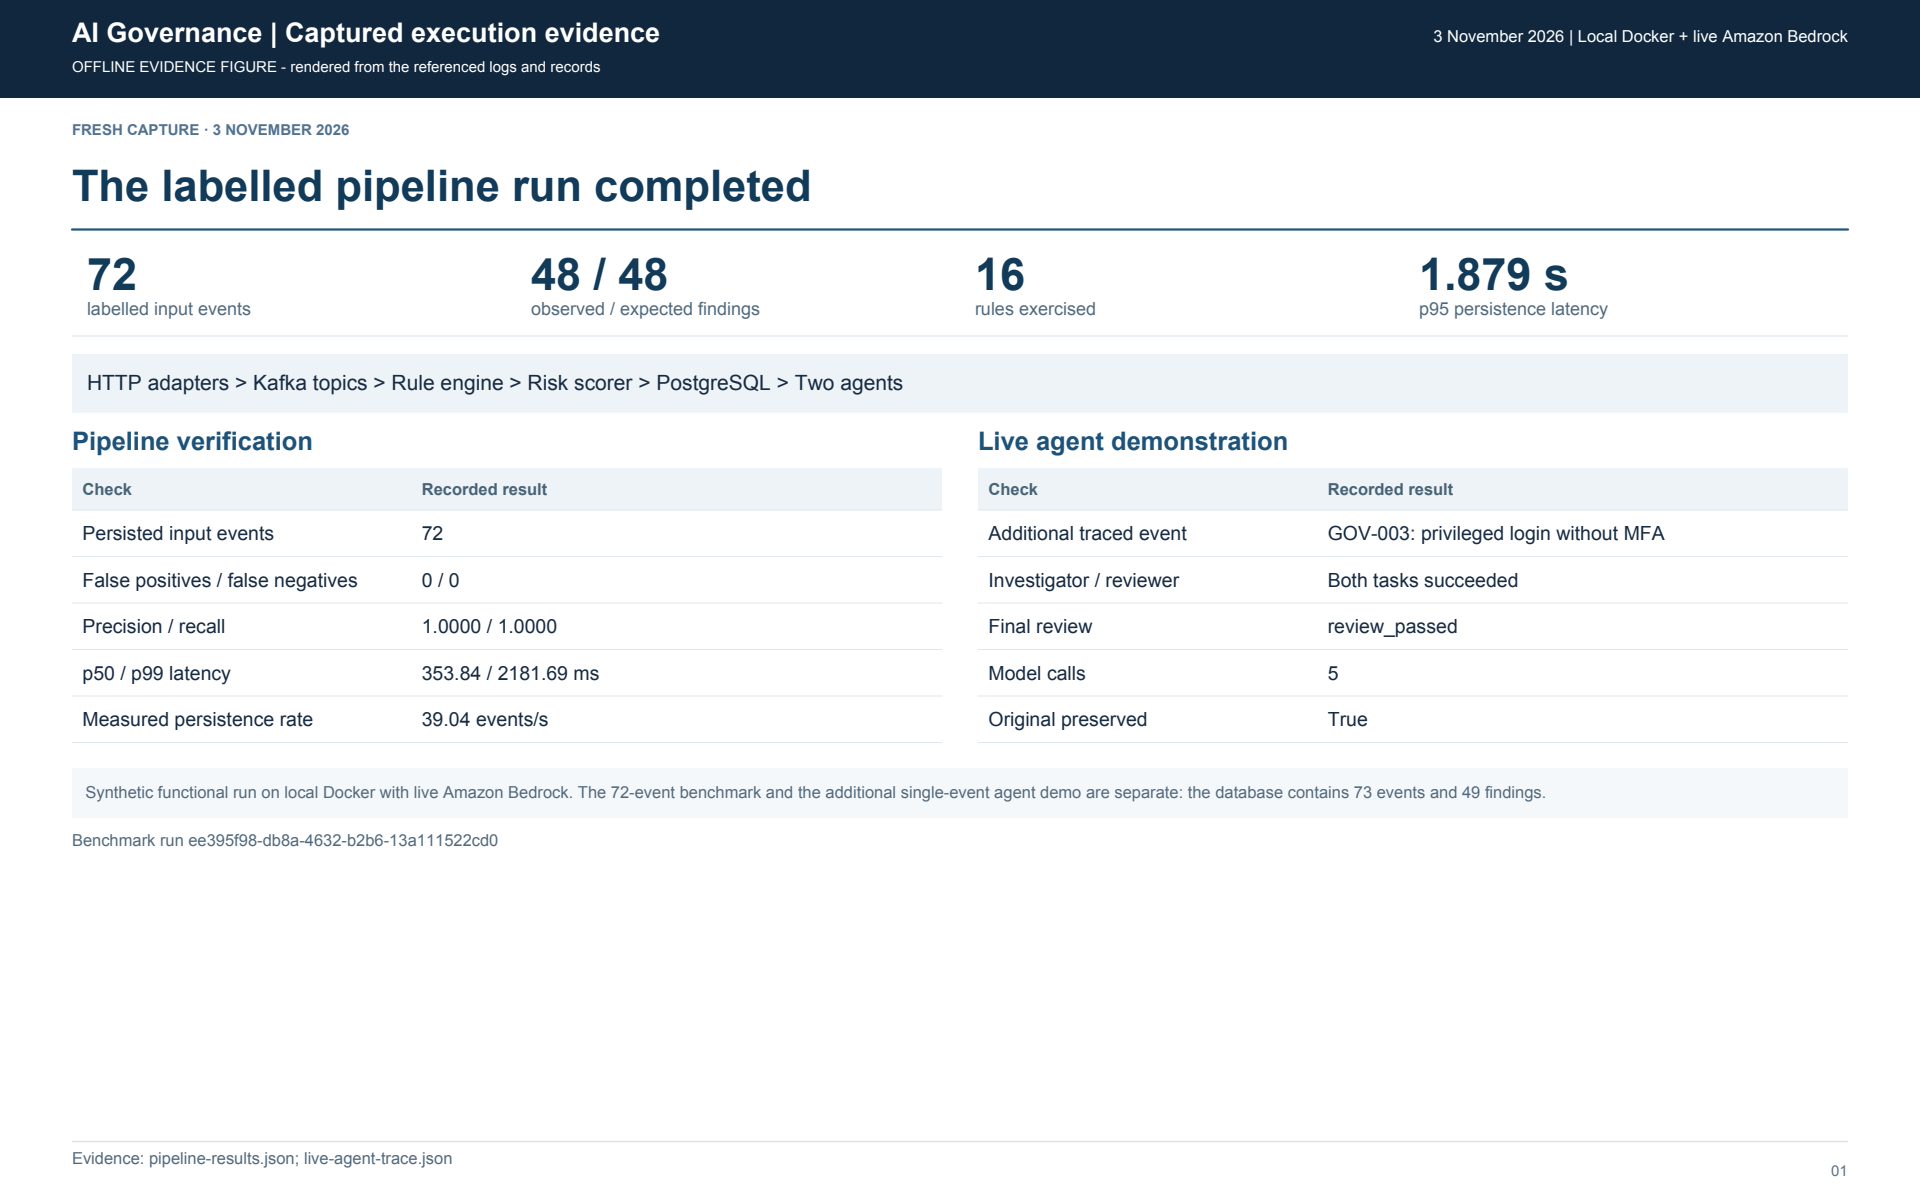
\includegraphics[width=\columnwidth]{figures/01-pipeline-run.png}
\caption{Labelled pipeline run used for functional evaluation.}
\label{fig:pipeline-run}
\end{figure}

\begin{figure}[t]
\centering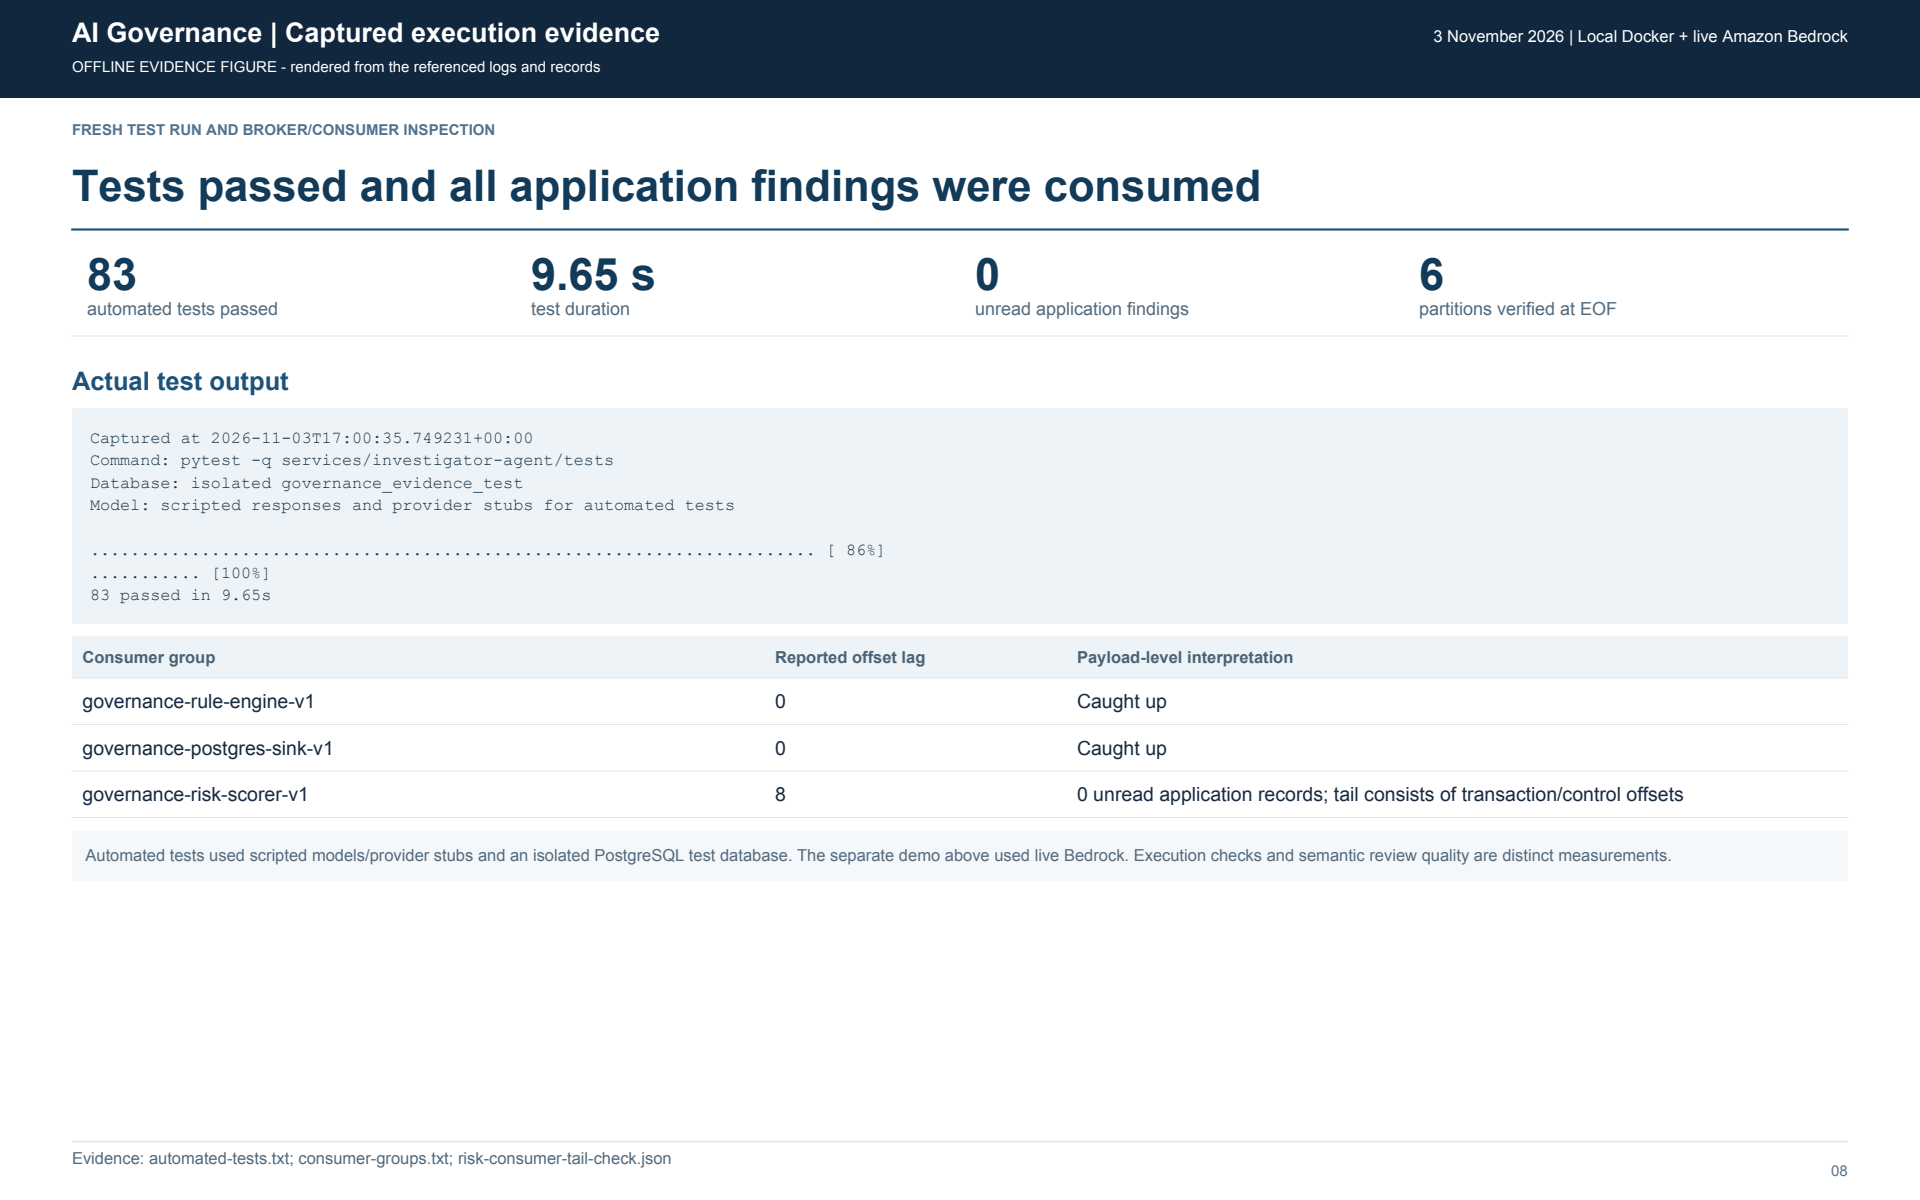
\includegraphics[width=\columnwidth]{figures/08-tests-and-consumer-checks.png}
\caption{Automated tests and consumer-tail verification.}
\label{fig:tests}
\end{figure}

\begin{figure}[t]
\centering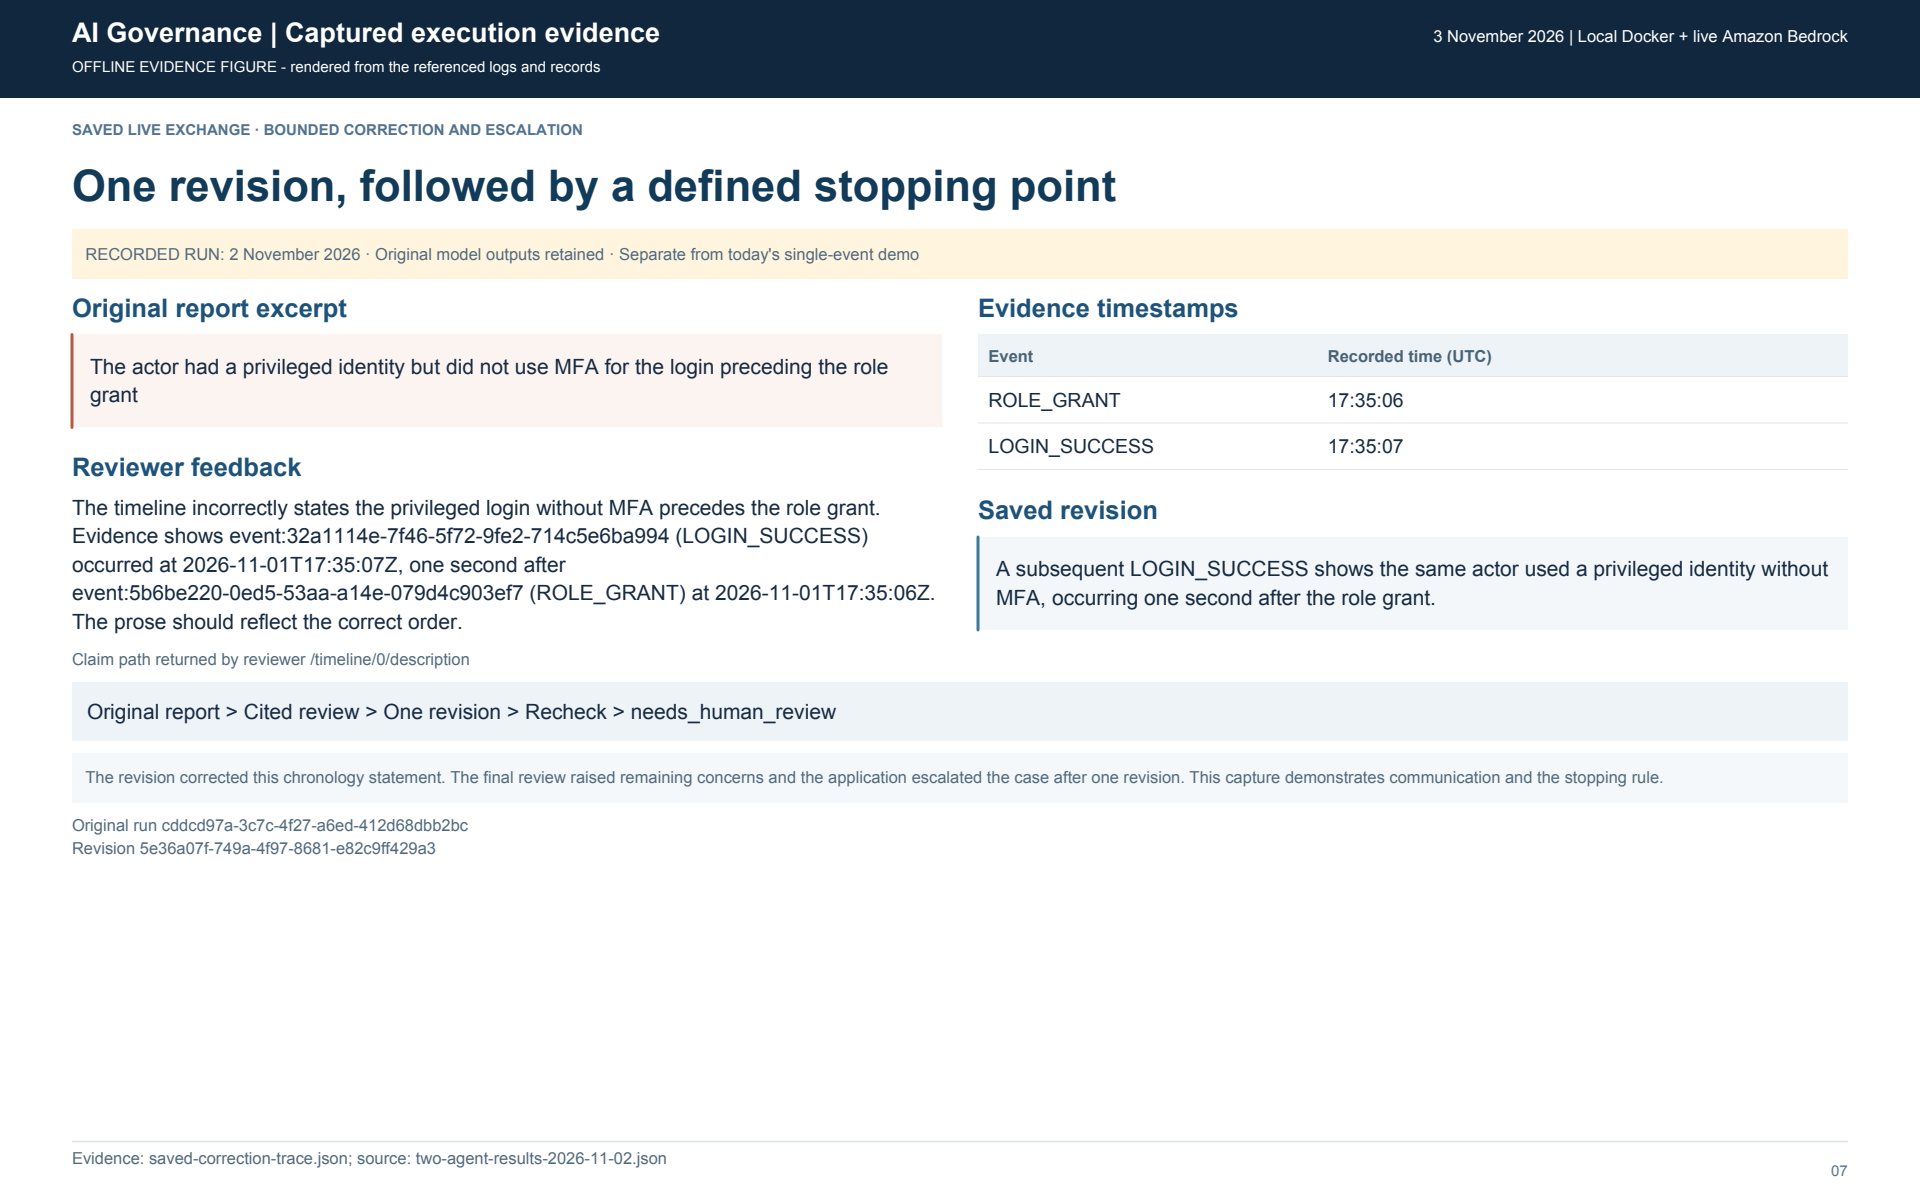
\includegraphics[width=\columnwidth]{figures/07-correction-and-recheck.png}
\caption{Bounded correction, recheck, and human-escalation evidence.}
\label{fig:correction}
\end{figure}

\begin{figure}[t]
\centering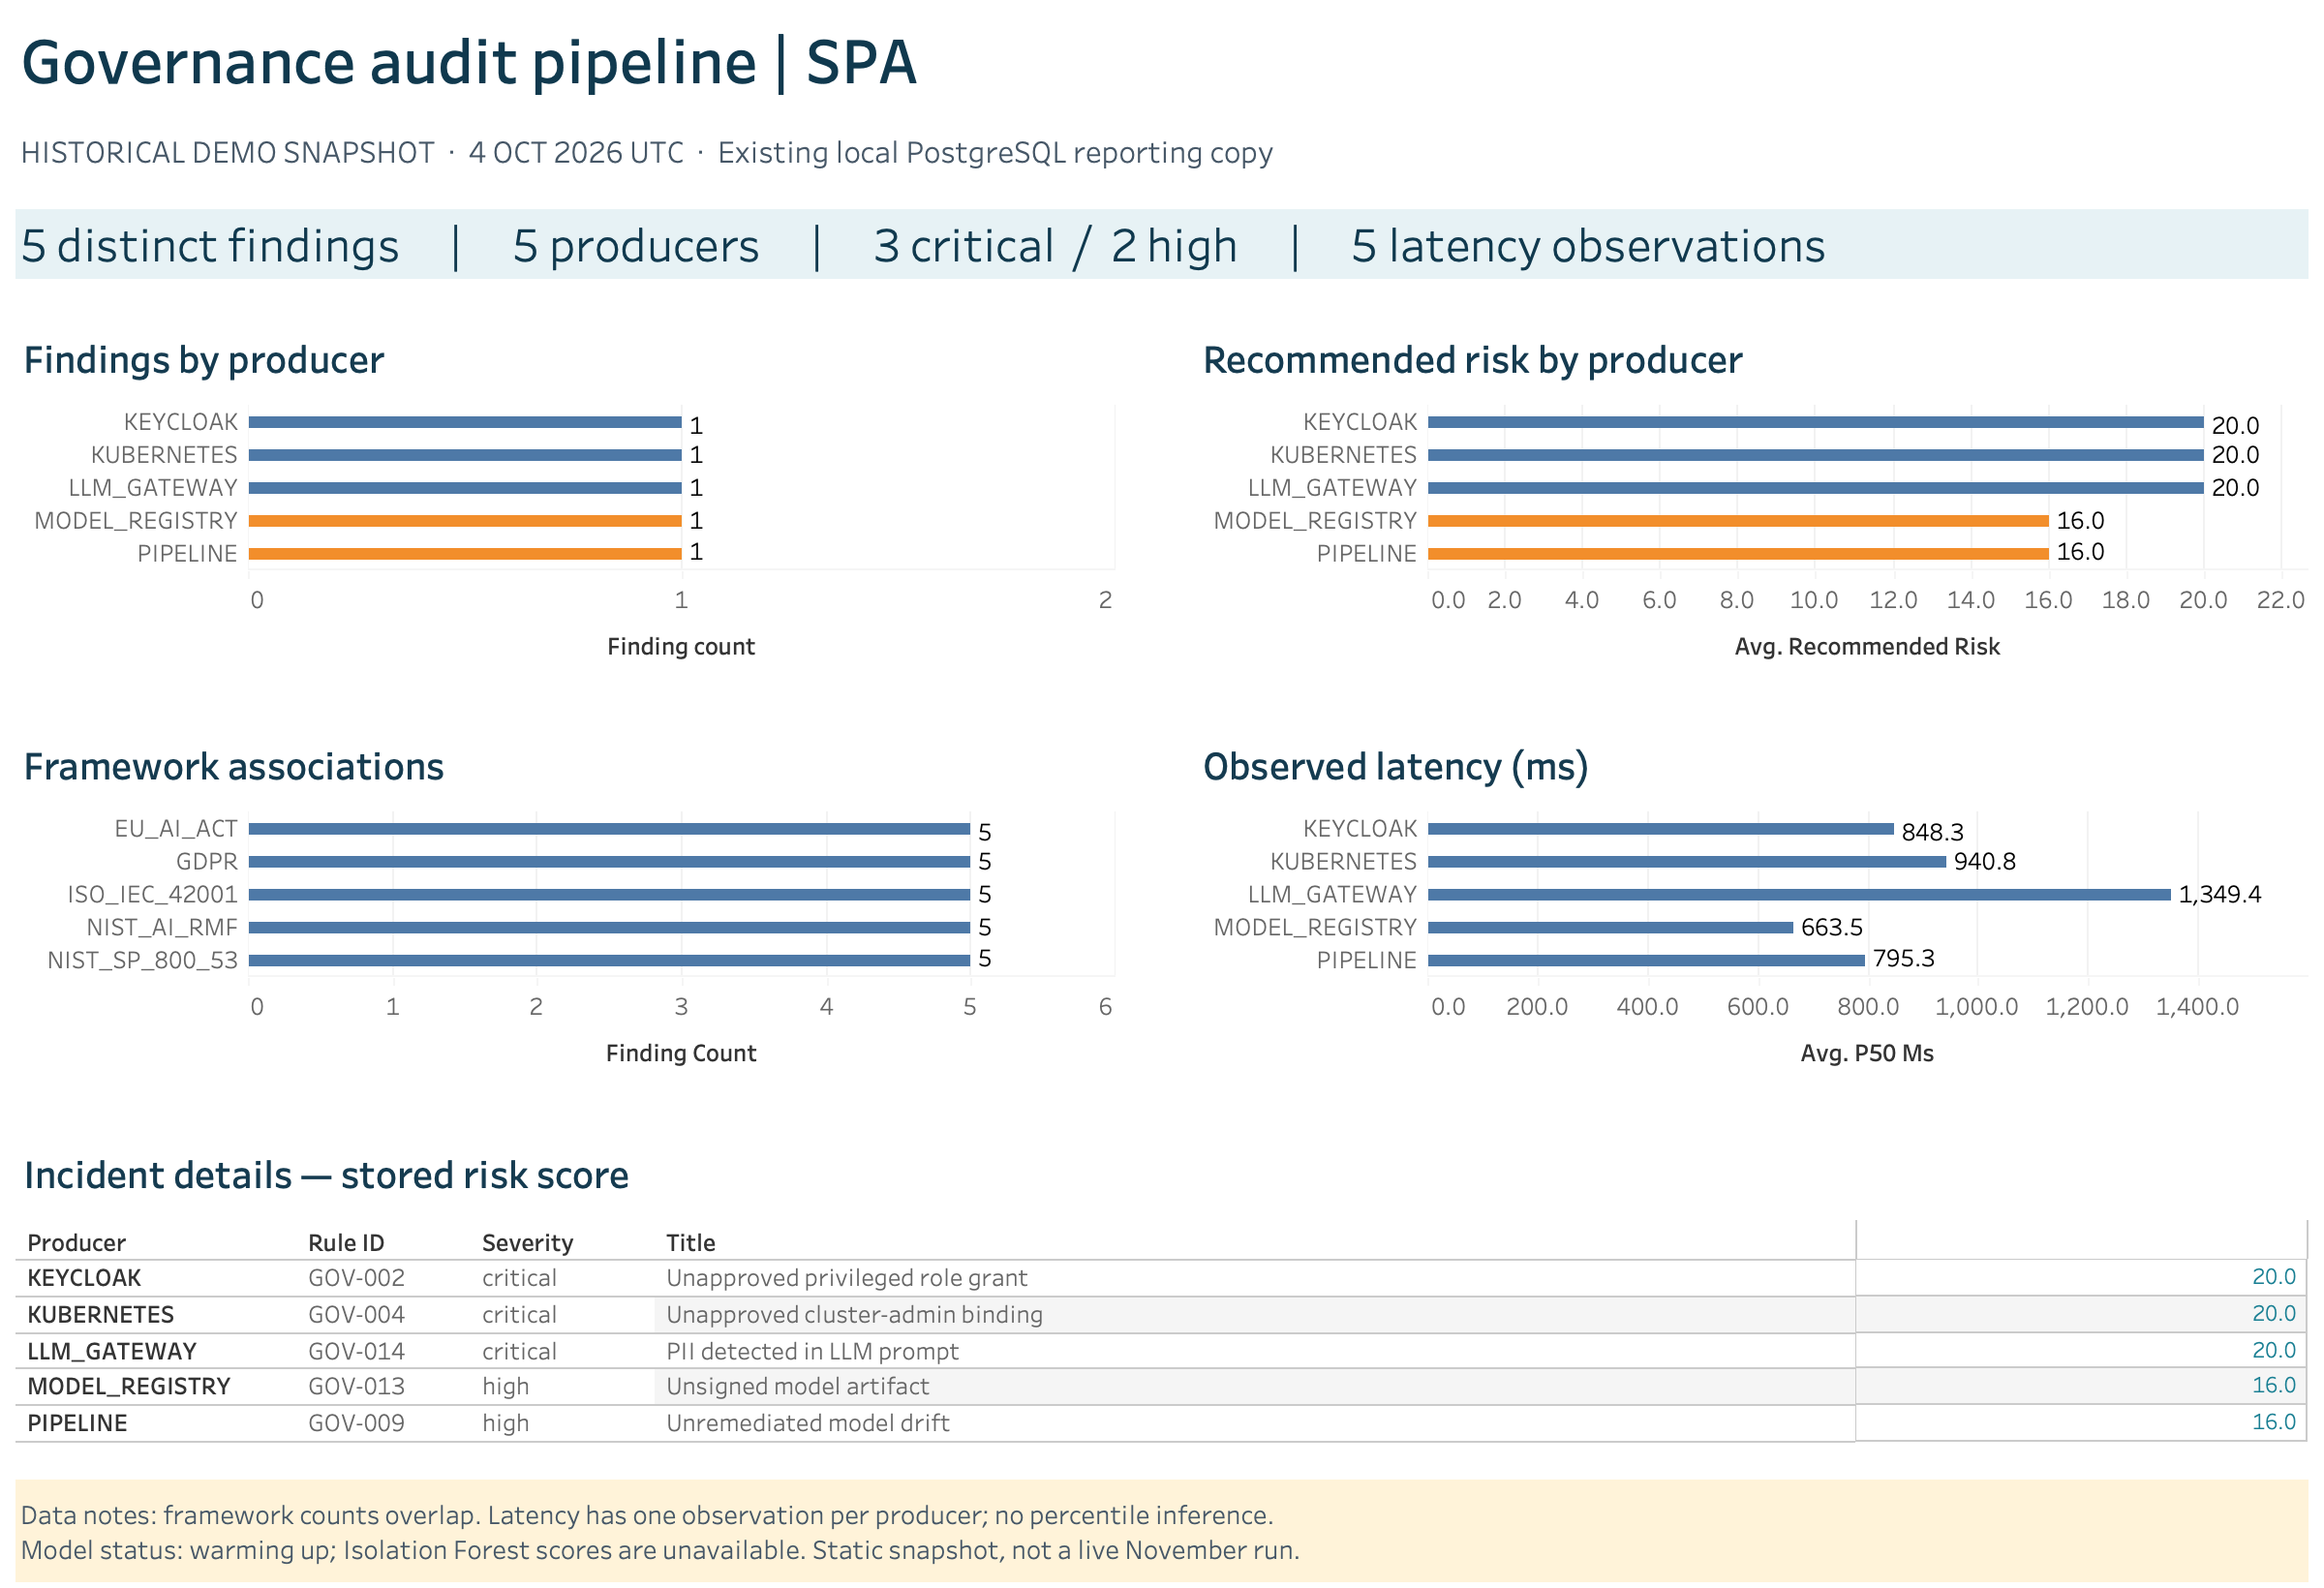
\includegraphics[width=\columnwidth]{figures/09-tableau-dashboard.png}
\caption{Operational governance dashboard for findings, risk, and latency.}
\label{fig:dashboard}
\end{figure}

\section{Discussion and Limitations}
The evaluation indicates that the topology recovered all expected findings under the documented baseline and fault-injection demonstrations. The architecture's strongest property is traceability: a source event can be followed through a rule, finding key, score, database record, evidence snapshot, and review state. Kafka's topic and consumer-group boundaries also provide operational separation that is difficult to obtain from direct service-to-service calls.

There are important limitations. The workload is small and source-shaped; it does not establish production throughput or broad semantic quality. The Isolation Forest is a comparative signal trained on recent findings, not a validated detector for every governance domain. Agent quality is shown through selected investigation and review traces, not a corpus-wide evaluation. Framework mappings are routing metadata and do not constitute legal advice or certification. Finally, cloud screenshots demonstrate captured resource and service states but do not replace a production readiness review.

\section{Reproducibility and Threats to Validity}
The repository is organized so that the principal claims in this paper can be inspected against source and evidence. Java topology code, Python services, SQL migrations, Docker Compose files, Kubernetes manifests, Terraform definitions, evaluation scripts, and captured screenshots are kept as separate artefacts. The local path can be executed with the supplied environment template and Compose configuration; the evaluation harness then injects labelled events and exports results. This makes the reported finding counts auditable at the level of source event, rule, output key, and persisted row.

There are four main threats to validity. First, the labelled workload is synthetic and small. A perfect precision and recall result on 72 events cannot establish behaviour for the full diversity of enterprise governance activity. Second, the throughput and latency observations are workload-specific and depend on the local execution profile, broker, database, and timing of the persistence interval. Third, the Isolation Forest is an unsupervised comparison model whose usefulness depends on the distribution and quality of the recent finding history. It should not be treated as a calibrated probability or legal risk estimate. Fourth, the agent evaluation covers selected investigation, correction, and reviewer traces rather than a broad benchmark of factuality, citation completeness, or adversarial robustness.

The system also has scope boundaries. It does not automatically remediate infrastructure, approve a model, or certify an organization. Framework labels route findings to relevant governance concepts; they do not replace legal interpretation. Cloud screenshots show captured infrastructure and service state, but deployment correctness still depends on account configuration, secrets, network policy, image provenance, and operational review. These constraints are intentional: an auditable reference implementation should state what its evidence demonstrates and what it does not demonstrate.

\begin{table}[t]\caption{Reproducibility artefacts and validity boundaries}\label{tab:validity}\centering\scriptsize\begin{tabular}{p{1.75cm}p{2.5cm}p{2.15cm}}\toprule\textbf{Area} & \textbf{Artefact} & \textbf{Boundary}\\\midrule Source behaviour & Producer adapters and mapper tests & Synthetic source-shaped events\\ Stream processing & Java topology tests and evaluator & Small labelled workload\\ Persistence & SQL migrations and sink tests & Environment-dependent database timing\\ Operations & Compose, Kubernetes, Terraform & Local and captured cloud profiles\\ Agents & Investigator/reviewer records & Selected traces, not corpus-wide quality\\\bottomrule\end{tabular}\end{table}

\section{Conclusion}
This paper presented a traceable real-time AI governance audit pipeline that joins heterogeneous event ingestion, Kafka Streams processing, risk scoring, PostgreSQL evidence, Tableau reporting, and bounded agent review. The implementation demonstrates how governance principles can be connected to executable controls and durable evidence without treating an LLM agent as an approval authority. The documented evaluation recovered 48 expected findings from 72 events across sixteen rules under baseline and recovery scenarios.

Future work includes larger semantic-quality benchmarks for agents, schema compatibility testing across releases, alerting for stale Kubernetes metrics APIs, governed evidence retention, multi-region disaster recovery, continuous dashboard validation, and approval workflows for framework-mapping changes. A larger labelled corpus would enable calibration beyond the current demonstration workload.

\section*{Acknowledgment}
The authors acknowledge the RV College of Engineering Department of Artificial Intelligence and Machine Learning for the academic setting in which this project was developed.

\begin{thebibliography}{20}
\bibitem{project} A. Ranjan, A. Gupta, and G. N. Naidu, ``AI-Governance-Audit-Pipeline,'' GitHub repository, 2026.
\bibitem{nist} E. Tabassi, ``Artificial Intelligence Risk Management Framework (AI RMF 1.0),'' NIST AI 100-1, 2023.
\bibitem{genai} NIST, ``Artificial Intelligence Risk Management Framework: Generative Artificial Intelligence Profile,'' NIST AI 600-1, 2024.
\bibitem{iso} ISO/IEC, ``ISO/IEC 42001:2023 Information technology--Artificial intelligence--Management system,'' 2023.
\bibitem{oecd} OECD, ``OECD AI Principles,'' updated 2024.
\bibitem{unesco} UNESCO, ``Recommendation on the Ethics of Artificial Intelligence,'' 2021.
\bibitem{eu} European Parliament and Council, ``Regulation (EU) 2024/1689 (Artificial Intelligence Act),'' 2024.
\bibitem{owasp} OWASP Foundation, ``OWASP Top 10 for Large Language Model Applications,'' 2025.
\bibitem{atlas} MITRE, ``MITRE ATLAS: Adversarial Threat Landscape for Artificial-Intelligence Systems,'' 2024.
\bibitem{saif} Google, ``Secure AI Framework (SAIF),'' 2023.
\bibitem{scorecard} OpenSSF, ``Open Source Security Foundation Scorecard Documentation,'' 2024.
\bibitem{kafka} Apache Software Foundation, ``Kafka Streams Developer Guide,'' 2024.
\bibitem{kube} Kubernetes Authors, ``Kubernetes Documentation: Workloads, Probes, Scaling and Disruptions,'' 2024.
\bibitem{rag} Y. Gao et al., ``Retrieval-Augmented Generation for Large Language Models: A Survey,'' arXiv:2312.10997, revised 2024.
\bibitem{agents} M. Wang et al., ``A Survey on Large Language Model based Autonomous Agents,'' arXiv:2308.11432, revised 2024.
\bibitem{scikit} scikit-learn Developers, ``IsolationForest API Reference,'' version 1.5, 2024.
\bibitem{otel} OpenTelemetry Authors, ``OpenTelemetry Documentation,'' 2024.
\bibitem{terraform} HashiCorp, ``Terraform AWS Provider Documentation,'' 2024.
\bibitem{bedrock} Amazon Web Services, ``Amazon Bedrock User Guide: Agents,'' 2025.
\bibitem{cloudwatch} Amazon Web Services, ``Monitor Amazon Bedrock Agents using CloudWatch Metrics,'' 2025.
\end{thebibliography}

\end{document}
